\subsection{Inteligencia Artficial}
Definir a la inteligencia artificial llega a ser complicado, esto debido a la dificultad que se tiene en definir lo que en verdad es inteligencia. Algunos grandes personajes pensaban de la inteligencia como la ambición, mientras que otros mencionaban a la imaginación como gran impulsador de la inteligencia. También lo consideraban como la capacidad de adaptarse a los cambios. Estas definiciones hacen pensar que no existe un consenso claro de lo que es la inteligencia, menos aun de la inteligencia artificial; sin embargo, en términos generales, se puede calificar de “inteligencia artificial” a todo aquel sistema sintético que muestra algún tipo de comportamiento “inteligente”. Esto quiere decir que se puede considerar como IA a todo a aquellos que simule los sentidos naturales como el visión o audición, incluso a la capacidad de algunos sistemas de aprender de forma autónoma según su entorno lo requiera. \parencite{bk_hurbans2020grokking}

\subsection{Perceptrón}
Inventado por Frank Rosenblatt en 1957, el Perceptrón es la unidad básica de una red neuronal e incluso es considerado como la más simple red neuronal artificial (ANN). \parencite{bk_geron2022handml}

\begin{figure}[H]
	\begin{center}
		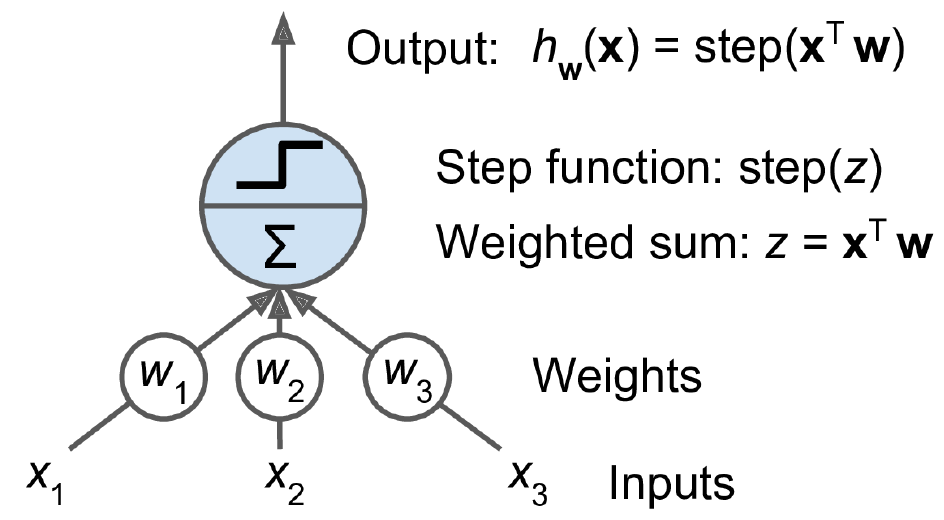
\includegraphics[width=1.00\textwidth]{2/figures/perceptron.png}
		\caption[Perceptrón]{Perceptrón. \\
		Fuente: \cite{bk_geron2022handml}. \textit{Hands-on machine learning with Scikit-Learn, Keras, and TensorFlow}.}
		\label{2:fig207}
	\end{center}
\end{figure}


\subsection{Perceptrón Multicapa}
Un Multi-Layer Perceptron (MLP) consiste en la unión de varios perceptrones, con la característica de estar organizados por capas. Existe una capa de entrada y otra de salida, todas las capas, a excepción de la salida, contiene una neurona adicional llamada bias. \parencite{bk_geron2022handml}

\begin{figure}[H]
	\begin{center}
		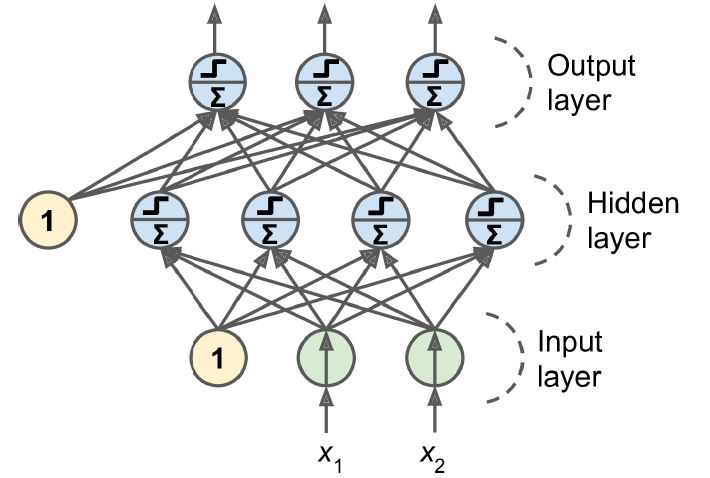
\includegraphics[width=1.00\textwidth]{2/figures/mlp.png}
		\caption[Perceptrón multicapa]{Perceptrón multicapa. \\
		Fuente: \cite{bk_geron2022handml}. \textit{Hands-on machine learning with Scikit-Learn, Keras, and TensorFlow}.}
		\label{2:fig208}
	\end{center}
\end{figure}


\subsection{Machine Learning}
El Aprendizaje Automático o Machine Learning es considerado como una ciencia y arte de dar instrucciones a una computadora para que pueda aprender por sí sola de una data. \parencite{bk_geron2022handml}

A continuación, se presenta el enfoque tradicional del Machine Learning.

\begin{figure}[H]
	\begin{center}
		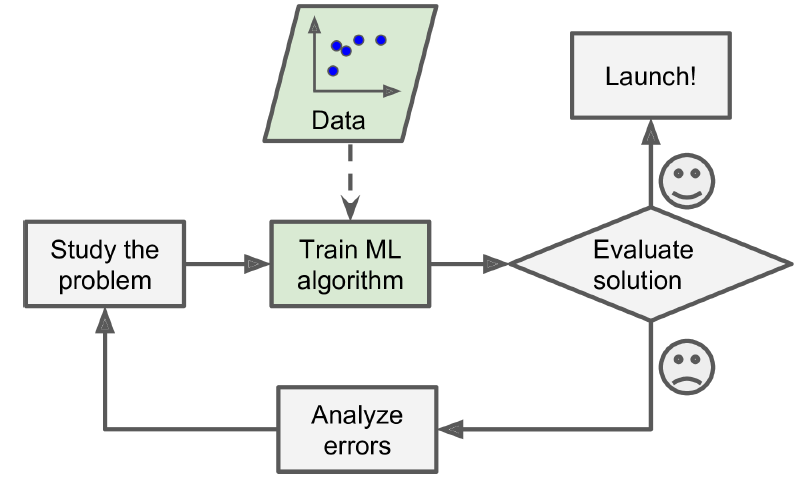
\includegraphics[width=1.00\textwidth]{2/figures/enfoque_ml.png}
		\caption[Enfoque del Machine Learning]{Enfoque del Machine Learning. \\
		Fuente: \cite{bk_geron2022handml}. \textit{Hands-on machine learning with Scikit-Learn, Keras, and TensorFlow}.}
		\label{2:fig209}
	\end{center}
\end{figure}

\subsection{Ecografía y las imágenes de ultrasonido}
Según \cite{pr_herrera2017diseimp}, la ecografía, que es una técnica de diagnóstico en donde se usan imágenes generadas por ultrasonido, es comúnmente desarrollado en las áreas de cardiología, ginecología, y otras más relacionadas. La popularidad de esta técnica se basa en la capacidad de las imágenes de alta calidad que se obtienen de este proceso, además de no ser un método invasivo o de radiación como muchos otros de su tipo.

\subsection{Transfer Learning}
\cite{bk_geron2022handml} nos menciona que el transfer learning o transferencia de aprendizaje es un técnica usada en el campo de Deep Learning que permite el uso de algunas capas de un modelo ya definido y entrenado previamente en un nuevo modelo que necesite ser entrenado en una tarea similar al que se desarrolla el modelo original. Las capas destinadas al reuso son normalmente las más cercanas a la entrada o también conocidas como capas inferiores. El beneficio de usar esta técnica radica en dos puntos importantes: cantidad de datos requeridos y velocidad de entrenamiento del modelo; es decir, la cantidad de datos que se deben usar para entrenar un modelo de alto desempeño se reduce considerablemente, mientras que el tiempo requerido para terminar este proceso es menor comparándolo a si lo entrenaran desde cero.

Para que esta técnica funcione debidamente, las capas más cercanas a la salida, conocidas también como capas de alto nivel, deben ser reemplazadas, esto debido a que son más específicas de las tareas del modelo original. Esto también incluye a la capa final, ya que posiblemente no tenga la cantidad de salidas necesarias para completar satisfactoriamente la nueva tarea.

A continuación se presenta de forma gráfica la técnica.

\begin{figure}[H]
	\begin{center}
		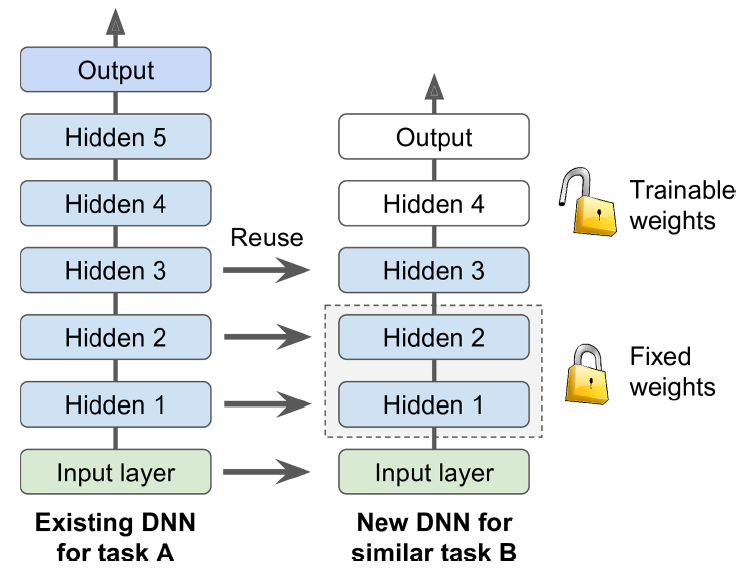
\includegraphics[width=1.00\textwidth]{2/figures/transfer_learning.PNG}
		\caption[Ejemplo de transfer learning]{Ejemplo de transfer learning. \\
		Fuente: \cite{bk_geron2022handml}. \textit{Hands-on machine learning with Scikit-Learn, Keras, and TensorFlow}.}
		\label{2:fig210}
	\end{center}
\end{figure}


\subsection{Data Augmentation}

Según \cite{bk_geron2022handml} el aumento de datos o data augmentation es una técnica de regularización que permite reforzar la cantidad de muestras en un conjunto de datos. Esto se realiza a través de la generación de nuevas instancias similares a los originales; es decir, las personas no deberían ser capaces de diferenciar una imagen generada de una del propio conjunto de datos.

Para generar estas nuevas muestras, normalmente se aplican diferentes transformaciones a las instancias del conjunto de datos original. Estas transformaciones pueden ser; por ejemplo, una simple rotación o recorte de la imagen, siempre y cuando no altere por completo su sentido como es el caso de voltear una imagen de texto de forma horizontal. 

El principal beneficio de esta técnica es que permite reducir el sobreajuste de los modelos entrenados. 

En la siguiente imagen se muestran algunas transformaciones que se pueden hacer al aplicar el aumento de datos. 

\begin{figure}[H]
	\begin{center}
		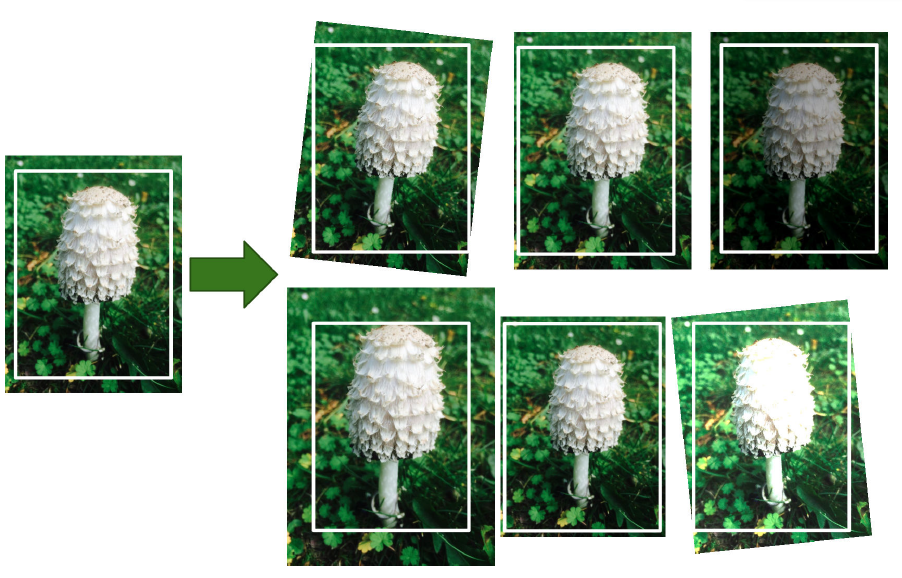
\includegraphics[width=1.00\textwidth]{2/figures/data_aug.PNG}
		\caption[Ejemplo de data augmentation]{Ejemplo de data augmentation. \\
		Fuente: \cite{bk_geron2022handml}. \textit{Hands-on machine learning with Scikit-Learn, Keras, and TensorFlow}.}
		\label{2:fig211}
	\end{center}
\end{figure}

